
% This LaTeX was auto-generated from MATLAB code.
% To make changes, update the MATLAB code and republish this document.

\documentclass{article}
\usepackage{graphicx}
\usepackage{color}

\sloppy
\definecolor{lightgray}{gray}{0.5}
\setlength{\parindent}{0pt}

\begin{document}

    
    \begin{verbatim}
clear all;
close all;


% -- Default matrix A  (you can change this matrix A !!)


A  =  [  2,-1,-1;
         -1,2,-1;
         -1,-1,2]


% -- Select the eigenvector to plot

eigvec_to_plot = 1;   % -- This is associated with:  lambda1 = 0
%eigvec_to_plot = 2;   % -- This is associated with:  lambda2 = 3
%eigvec_to_plot = 3;   % -- This is associated with:  lambda3 = 3


disp('The eigenvalues and eigenvectors of matrix A are:')
[V,D] = eig(A)

% -- Define cube

shift_x = 0;
shift_y = 0;
shift_z = 0;

x1 = [0 1 1 0 0 1 1 0] + shift_x;
x2 = [0 0 0 0 1 1 1 1] + shift_y;
x3 = [0 0 1 1 0 0 1 1] + shift_z;

% -- Define x
x = [x1;  x2;  x3];

% -- Calculate transformation
y = A*x;

% -- Housekeeping duties
xmin = -2;
xmax = 2;
ymin = -2;
ymax = 2;
zmin = -2;
zmax = 2;

% -- Plot data points (preimage and image)

figure

for count = 1:1:length(x1)
    preimage_handle(count) = plot3(x(1,count), x(2,count), x(3,count), '.');



    if count == 1
        set(preimage_handle(count), 'Color', 'red', 'MarkerSize', 50, 'Linewidth', 5);
    else

        set(preimage_handle(count), 'Color', 'black', 'MarkerSize', 15, 'Linewidth', 5);
    end
end


% --  Plot one face of the preimage and its corresponding image

preimageFace_handle(1) = patch(x(1, 1:4), x(2, 1:4), x(3, 1:4),  4);
preimageFace_handle(2) = patch(x(1, 5:8), x(2, 5:8), x(3, 5:8),  4);
preimageFace_handle(3) = patch(x(1, [1 4 8 5] ), x(2, [1 4 8 5]), x(3, [1 4 8 5]),  4);
preimageFace_handle(4) = patch(x(1, [1 2 6 5]), x(2, [1 2 6 5]), x(3, [1 2 6 5]),  4);

set(preimageFace_handle(1), 'FaceColor', 'blue', 'FaceAlpha', 1);
set(preimageFace_handle(2), 'FaceColor', 'green', 'FaceAlpha', 0.2);
set(preimageFace_handle(3), 'FaceColor', 'yellow', 'FaceAlpha', 0.2);
set(preimageFace_handle(4), 'FaceColor', 'red', 'FaceAlpha', 0.2);


% -- Emphasize the x, y, z-axexs
%line([0 xmax], [0 0], [0 0], 'Color', 'black', 'Linestyle', '-.', 'Linewidth', 2);  % -- x-axis
%line([0 0], [0 ymax], [0 0], 'Color', 'black', 'Linestyle', '-', 'Linewidth', 2);  % -- y-axis
%line([0 0], [0 0], [0 zmax], 'Color', 'black', 'Linestyle', 'x', 'Linewidth', 2);  % -- z-axis

eig_scale = 3;
% -- Plot eigenvector #2
line('XData', eig_scale.*[0 V(1,eigvec_to_plot)], 'YData', eig_scale.*[0 V(2,eigvec_to_plot)], 'ZData', eig_scale.*[0 V(3,eigvec_to_plot)], 'Color', 'black', 'Linestyle', '-.', 'Linewidth', 2);

axis square;
grid on;
xlabel('x-axis', 'FontName', 'Arial', 'FontSize', 15);
ylabel('y-axis', 'FontName', 'Arial', 'FontSize', 15);
zlabel('z-axis', 'FontName', 'Arial', 'FontSize', 15);
axis([xmin  xmax  ymin  ymax  zmin  zmax]   );
hold off
title('The pre-image before transformation by A')



% \\\\\\\\\\\\\\\\\\\\\\\\\\\\\\\\\\\\\\\\\\\\\\\\\\\\
%   Figure 2:  Plot the transformed image
% \\\\\\\\\\\\\\\\\\\\\\\\\\\\\\\\\\\\\\\\\\\\\\\\

xmin2 = -5;
xmax2 = 5;
ymin2 = -5;
ymax2 = 5;
zmin2 = -5;
zmax2 = 5;


figure

for count = 1:1:length(x1)
    %preimage_handle(count) = plot3(x(1,count), x(2,count), x(3,count), '.');
    %hold on;
    image_handle(count) = plot3(y(1,count), y(2,count), y(3,count), 'o');
    hold on;

    if count == 1
            %set(preimage_handle(count), 'Color', 'red', 'MarkerSize', 50, 'Linewidth', 5);
            set(image_handle(count), 'Color', 'red', 'MarkerSize', 30, 'Linewidth', 1);
    else

        %set(preimage_handle(count), 'Color', 'black', 'MarkerSize', 15, 'Linewidth', 5);
        set(image_handle(count), 'Color', 'black', 'MarkerSize', 10, 'Linewidth', 5);
    end
end


% --  Plot one face of the preimage and its corresponding image

% preimageFace_handle(1) = patch(x(1, 1:4), x(2, 1:4), x(3, 1:4),  4);
% preimageFace_handle(2) = patch(x(1, 5:8), x(2, 5:8), x(3, 5:8),  4);
% preimageFace_handle(3) = patch(x(1, [1 4 8 5] ), x(2, [1 4 8 5]), x(3, [1 4 8 5]),  4);
% preimageFace_handle(4) = patch(x(1, [1 2 6 5]), x(2, [1 2 6 5]), x(3, [1 2 6 5]),  4);
%
% set(preimageFace_handle(1), 'FaceColor', 'blue', 'FaceAlpha', 1);
% set(preimageFace_handle(2), 'FaceColor', 'green', 'FaceAlpha', 0.2);
% set(preimageFace_handle(3), 'FaceColor', 'yellow', 'FaceAlpha', 0.2);
% set(preimageFace_handle(4), 'FaceColor', 'red', 'FaceAlpha', 0.2);

imageFace_handle(1) = patch(y(1, 1:4), y(2, 1:4), y(3, 1:4),  4);
imageFace_handle(2) = patch(y(1, 5:8), y(2, 5:8), y(3, 5:8),  4);
imageFace_handle(3) = patch(y(1, [1 4 8 5]), y(2, [1 4 8 5]), y(3, [1 4 8 5]),  4);
imageFace_handle(4) = patch(y(1, [1 2 6 5]), y(2, [1 2 6 5]), y(3, [1 2 6 5]),  4);

set(imageFace_handle(1), 'FaceColor', 'blue', 'FaceAlpha', 0.2);
set(imageFace_handle(2), 'FaceColor', 'green', 'FaceAlpha', 0.2);
set(imageFace_handle(3), 'FaceColor', 'yellow', 'FaceAlpha', 0.2);
set(imageFace_handle(4), 'FaceColor', 'red', 'FaceAlpha', 0.2);


% -- Emphasize the x, y, z-axexs
%line([0 xmax], [0 0], [0 0], 'Color', 'black', 'Linestyle', '-.', 'Linewidth', 2);  % -- x-axis
%line([0 0], [0 ymax], [0 0], 'Color', 'black', 'Linestyle', '-', 'Linewidth', 2);  % -- y-axis
%line([0 0], [0 0], [0 zmax], 'Color', 'black', 'Linestyle', 'x', 'Linewidth', 2);  % -- z-axis

eig_scale = 3;
% -- Plot eigenvector #2
line('XData', eig_scale.*[0 V(1,eigvec_to_plot)], 'YData', eig_scale.*[0 V(2,eigvec_to_plot)], 'ZData', eig_scale.*[0 V(3,eigvec_to_plot)], 'Color', 'black', 'Linestyle', '-.', 'Linewidth', 2);

axis square;
grid on;
xlabel('x-axis', 'FontName', 'Arial', 'FontSize', 15);
ylabel('y-axis', 'FontName', 'Arial', 'FontSize', 15);
zlabel('z-axis', 'FontName', 'Arial', 'FontSize', 15);
axis([xmin2  xmax2  ymin2  ymax2  zmin2  zmax2]   );
hold off
title('The image:  Post-transformed by A')
\end{verbatim}

        \color{lightgray} \begin{verbatim}
A =

     2    -1    -1
    -1     2    -1
    -1    -1     2

The eigenvalues and eigenvectors of matrix A are:

V =

    0.5774    0.3000    0.7594
    0.5774   -0.8076   -0.1199
    0.5774    0.5077   -0.6395


D =

     0     0     0
     0     3     0
     0     0     3

\end{verbatim} \color{black}
    
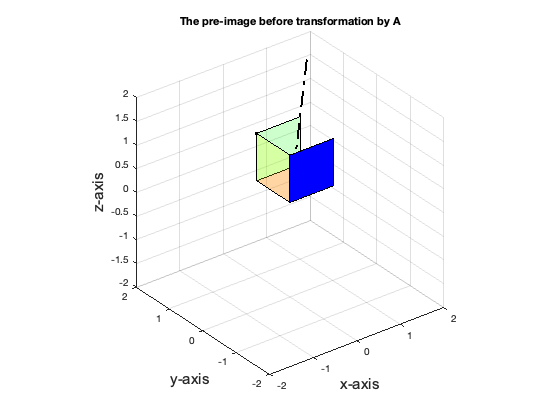
\includegraphics [width=4in]{Problem5_transformation_01.png}

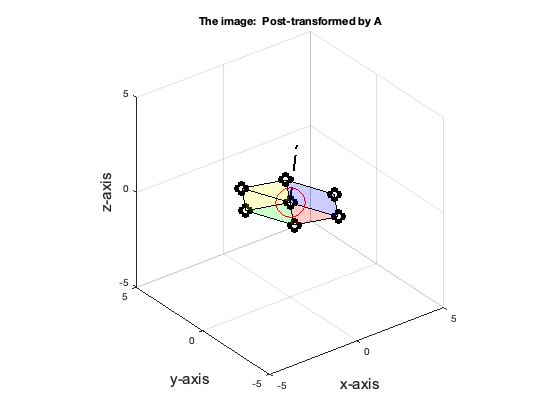
\includegraphics [width=4in]{Problem5_transformation_02.png}



\end{document}

